\section{\methodname{} Model Architecture} \label{sec:model}


\begin{figure}[t!]
    \centering
    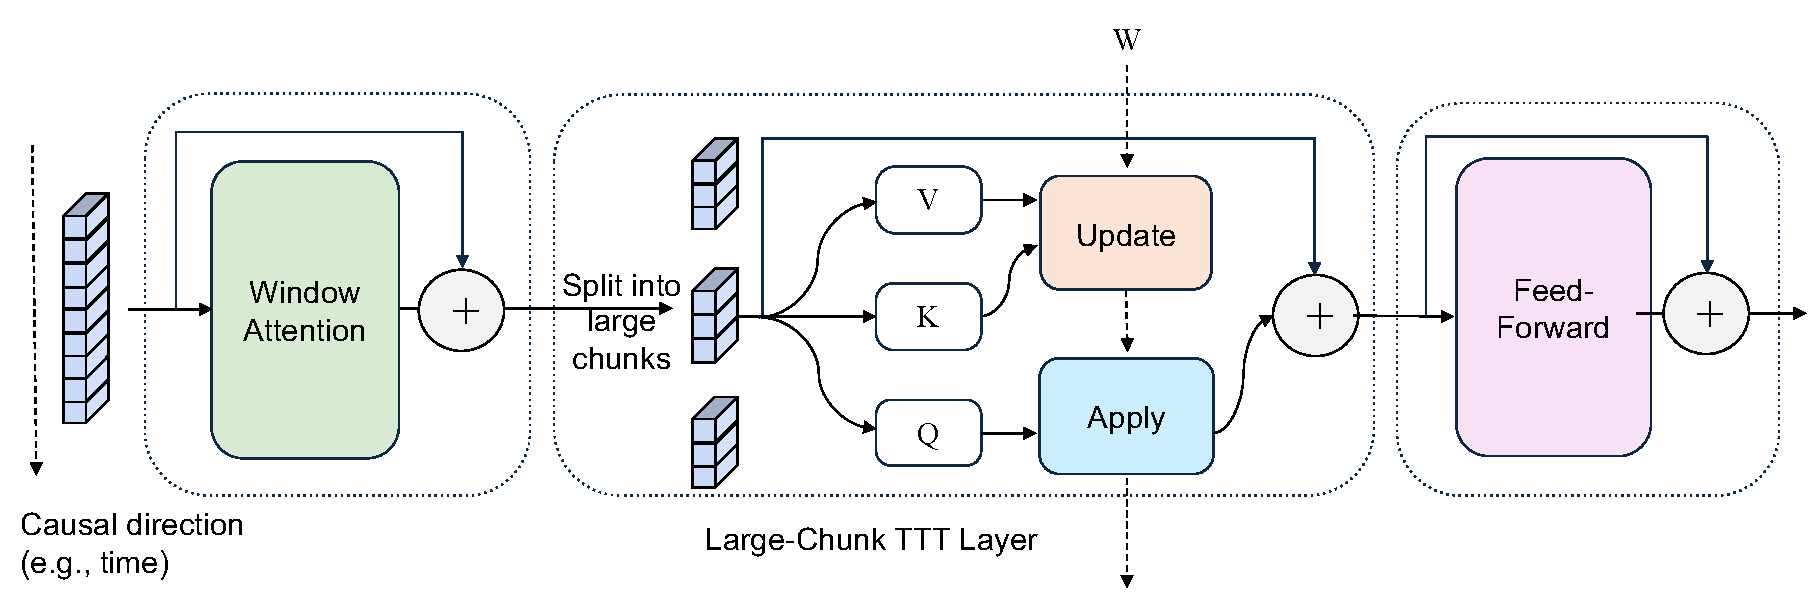
\includegraphics[width=1.0\textwidth]{figures/lact_model_arch_v3.pdf}
    \vspace{-0.20in}
    \caption{The basic diagram for a \methodname{} block. 
    The large-chunk TTT layer updates the fast weight $W$ to store historical context information,
    while the window attention handles the locality and internal structures within the chunk. 
    The solid line denotes the information flow over model depth and the dashed line denotes the information flow over time (i.e., the fast weight $W$ passing through chunks).
    Various instantiations in Sec.~\ref{sec:method} use different chunk sizes and window attention types according to the specific data structure. Additionally, window attention and large-chunk TTT layers can be combined within the same layer by sharing the QKV and summing their outputs; this in-layer mixing is used in our language modeling and video generation experiments (see Appendix~\ref{alg:lact_hybrid} for such pseudocode).}
    \vspace{-0.10in}
    \label{fig:lact_model_arch}
\end{figure}

As shown in Fig.~\ref{fig:lact_model_arch},
\methodname{} block consists of three types of layers: a window attention layer, a large-chunk TTT layer, and a feed-forward layer.
Each layer is equipped with residual connections~\cite{he2015deep} following the practice in Transformer~\cite{vaswani2017attention}.
The window attention layer performs local self-attention 
to capture the local dependency.
In the TTT layer, we split the sequence into large chunks.
The history context is gradually compressed into the fast weights through an `update' operation (regarding key vectors $K$ and value $V$), and latest weight is `applied' to the current query vector (Q) for computing its corresponding output.
The feed-forward layer performs channel mixing as in Transformer.
We omit several linear and normalization layers in Fig.~\ref{fig:lact_model_arch} for clarity and details are in Appendix~\ref{sec:ttt_pseudocode}.
Our framework offer great flexibility in handling diverse data types. 
In this section, we 
present the general designs in our approach and later  describe data-specific variations 
in Sec.~\ref{sec:method}.



\subsection{Large-Chunk TTT Layer}
\label{sec:ttt_layer}
Different from the per-token update in Eqn.~\ref{eq:ttt_update}, the chunk-wise update computes the gradient of the summed loss over all keys $\{k_i\}$ and values $\{v_i\}$ within the chunk.
% chunk-wise update simply calculates the update based on the loss sum for all key $\{k_i\}_i$ and values $\{v_i\}_i$ in the chunk. 
% The update equation would be:
% \begin{equation}
% W \leftarrow W - \eta \nabla_{W} \sum_i \mathcal{L} \big(f_W(k_i), v_i\big),
% \label{eq:ttt_chunk_update}
% \end{equation}
% For such large-chunk design, 
As the chunk size is large, weight updates are performed infrequently. This enables more sophisticated weight-update rule designs (discussed in Sec.~\ref{sec:update_rule}) and amortizes the update cost.
% As the chunk-size is larger, the weight's update is performed less frequently. 
% Thus it allows more sophisticated design  of update rule (discussed later in Sec.~\ref{sec:update_rule}) and the update costs are amortized.
% which we will discuss later in Sec~\ref{sec:update_rule}.
% As we applied the large-chunk update, it can leverage 
% and the update rule is no longer constrained by the simple.
% Thus we also free the design of 
% More specifically, 
The `update' operation for the fast weight is:
\begin{align}
% g &=  \nabla_{W}  \sum_i \eta_i \mathcal{L} \big(f_W(k_i), v_i\big) \\
% W &\leftarrow \mathrm{update} (W, g),
g &=  \nabla_{W}  \sum_{i=1} ^b \eta_i \mathcal{L}  \big(f_W(k_i), v_i\big) \label{eq:ttt_chunk_gradient} \\
W &\leftarrow \mathrm{weight\mbox{-}update} (W, g),
\label{eq:ttt_chunk_update}
\end{align}
% \sai{
where $b$ is the chunk size, $g$ is the gradient of the fast-weight loss function, 
% \hao{
and $\eta_i$ is the learning rate of each token (usually predicted from input tokens).
The `apply' operation $o_i = f_W(q_i)$ is the same as Eqn.~\ref{eq:ttt_apply} and 
% we apply  the same updated fast weight $W$ to all query vectors $\{q_i\}$ in the chunk.
 all query vectors $\{q_i\}$ in the chunk share the same updated fast weight $W$.



% We also exclude the bias term for stability following the trend.
Motivated by recent 
% practice in 
LLMs~\cite{touvron2023llama}, we adopt SwiGLU-MLP~\cite{shazeer2020glu} without bias terms as the fast-weight 
network. 
Our fast weights consists of three weight matrix $W = \{W_1, W_2, W_3\}$, and the network 
is:
% as follows:
% the $f_W(x)$ defined as below with three sub-weight $W = \{W^1, W^2, W^3\}$ for the MLP.
% A full derivation of forward and backward can be found in Appendix.
\begin{equation}
f_W(x) = W_2 \left[ \mathrm{SiLU}(W_1 x) \circ (W_3 x) \right]
\label{eq:swiglu}
\end{equation}
where $\circ$ is an elementwise multiplication. 
% A detailed derivation for the forward and backward of the fast-weight function is in Appendix.
% For the loss function for the fast weight, we used a simple dot product loss between the output of fast weight network and the values.
We apply a simple dot product loss as our loss function:
\begin{align}
    \mathcal{L} \big(f_W(k_i), v_i\big) = -f_W(k_i)^\top v_i 
\label{eq:loss}
\end{align}
% Intuitively, the closer the two vectors are, the bigger the dot product is, and the lower the loss would be.
% We take several normalizations to improve the stability of the network, which also prevent the loss to be unbounded.
% We also involve extra normalization layers in the MLP to prevent the loss from being unbounded, and the full details are included in the Appendix.

\noindent\textbf{Execution orders for `apply' and `update'.
}
Note that the `update' operation and `apply' operation of TTT are decoupled,  
and we can set the chunk size adaptively and apply these operation in different 
orders; this allows us to model diverse kinds of data dependencies, similar to different 
attention masks in self-attention. 
% we can apply them in a specific order to certain chunks of data to model different data dependencies.
% To use such layer in a sequence of data, we consider 
% performing chunk-wise \textit{update} and \textit{apply} operations iteratively over a sequence. 
% It depends on the desired update rate and also causality of the data.
% Our algorithm treats each chunk as an unordered set, meaning that tokens within a chunk do not have a predefined order. 
% As fast weights are updated iteratively across a sequence of chunks, the algorithm implicitly views these chunks as a one-dimensional ordered sequence.  
% Thus, \methodname{} essentially models input data as sequences of sets. 
% \sai{I feel this sentence lacks a direct connection to the Figure.}
Figure~\ref{fig:large_chunk_recurrence} illustrates this concept.
In Figure~\ref{fig:large_chunk_recurrence}a, when the chunk size equals the full sequence length, performing the apply followed by the update operation is conceptually similar to full attention. 
Using update and apply alternately leads to 
% behaviors similar to attention with 
a block-wise causal mask (Fig.~\ref{fig:large_chunk_recurrence}b), where the block size corresponds to the chunk size.
Switching the order between the two operations results in the a shift in the mask (Fig.~\ref{fig:large_chunk_recurrence}c). 
This shifted mask 
% important as it does not have 
does not leak future information within the chunk and is important when building the full causal mask 
% in-chunk future information leakage and helps build the full causal mask 
in Language Modeling (Sec.~\ref{sec:method-lm}).
Moreover, only updating on a subset of chunks 
and applying to all
% performing the apply operation on all chunks
(Figure~\ref{fig:large_chunk_recurrence}d) is analogous to strided 
block-wise causal mask.
% \sai{
% Changing the order of the
% apply and update operations on each chunk leads to behaviors  
% similar to attention with block-wise causal mask (Fig.~\ref{fig:large_chunk_recurrence}b) or shifted block-wise
% causal masks (Figure.~\ref{fig:large_chunk_recurrence}c), where the block size corresponds to the chunk size.
% Moreover, by only applying update on a subset of chunks 
% and performing the apply operation on all chunks (Figure~\ref{fig:large_chunk_recurrence}d, it's analogous to strided 
% block-wise causal mask.
% }


% \hao{Mentioning about heads; as we will discuss in pararallelism and Video/Lang}



\begin{figure}[t!]
    \centering
    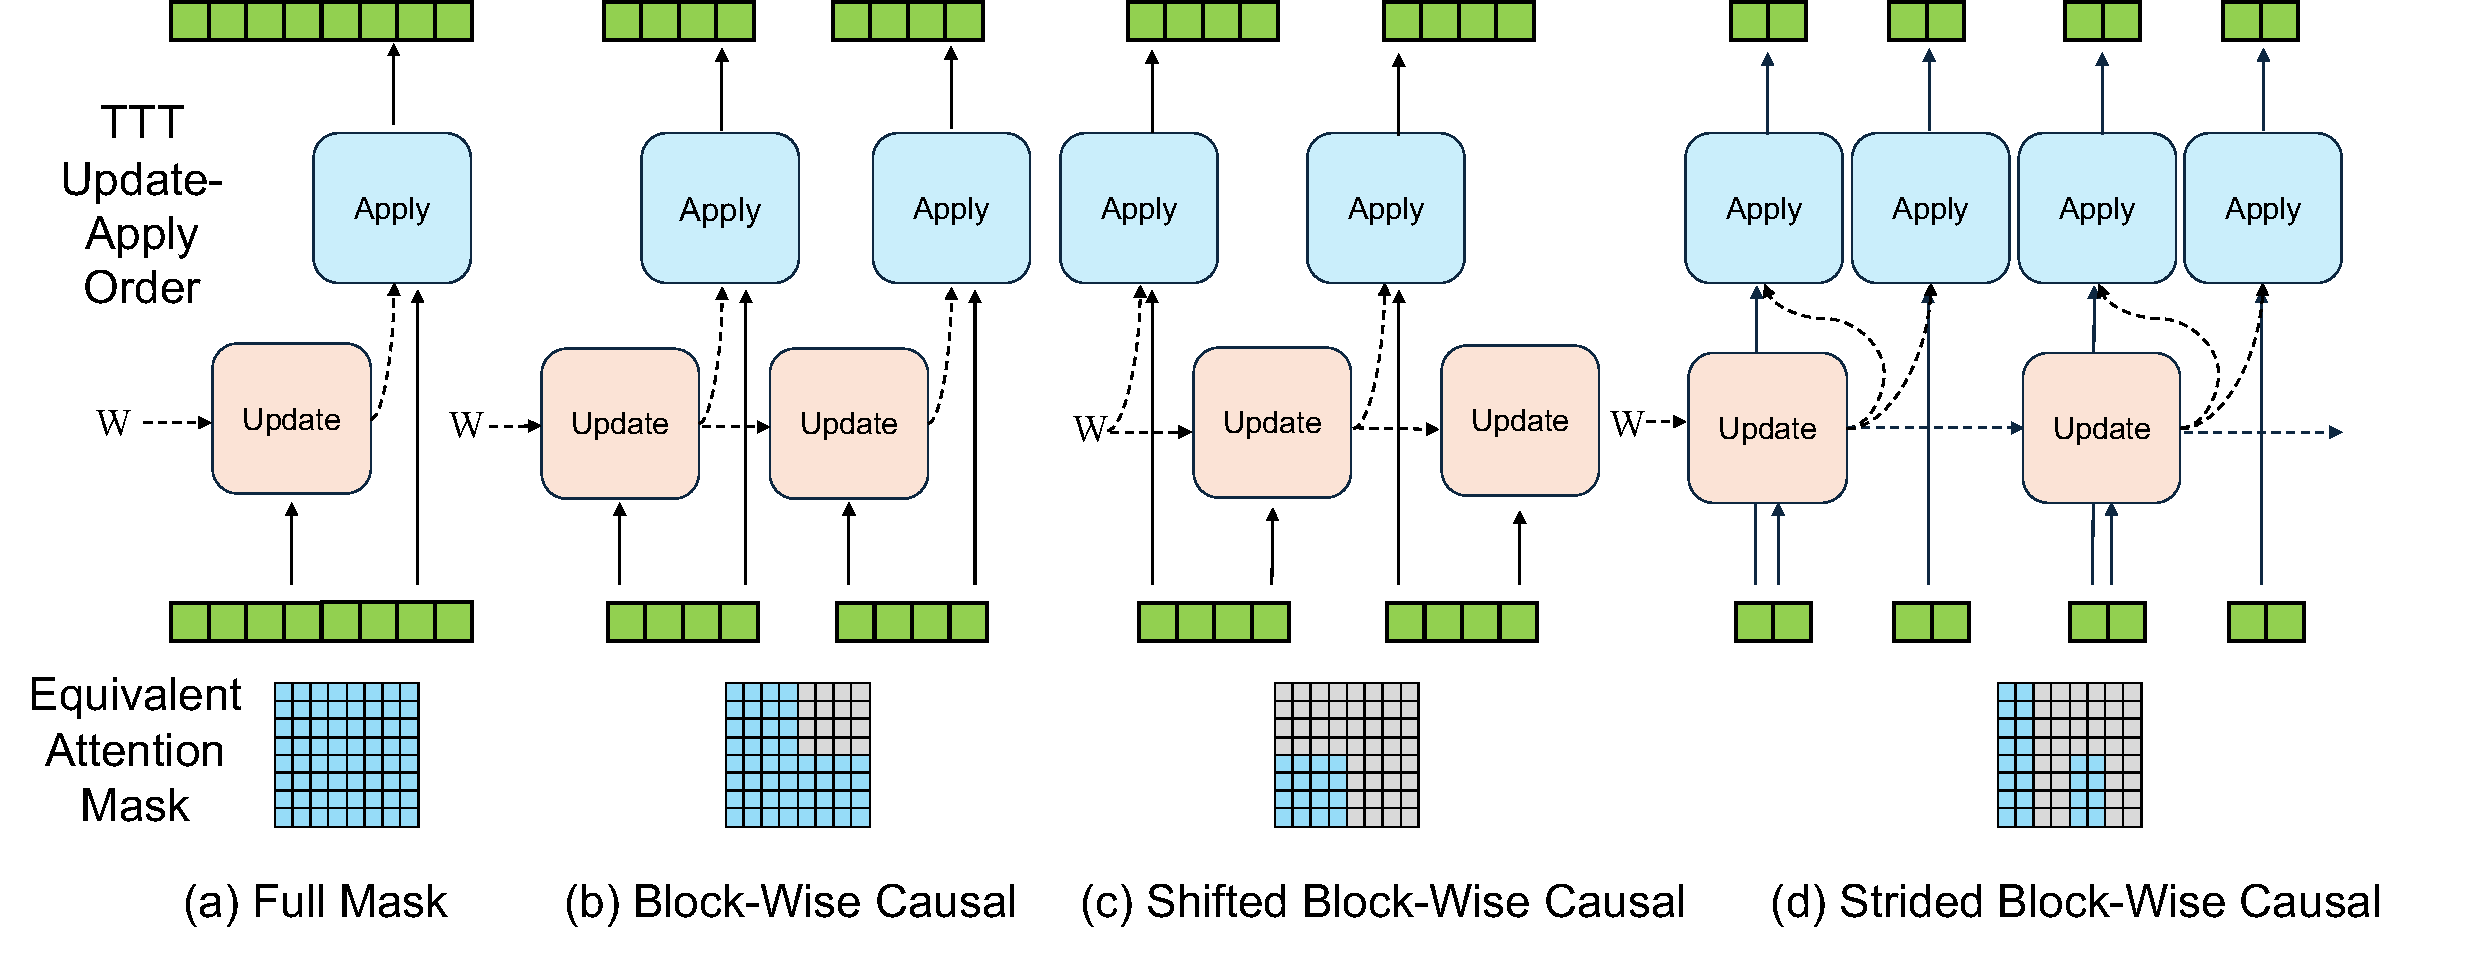
\includegraphics[width=1.0\textwidth]{figures/figure_chunk_mask_v3.pdf}
    \vspace{-0.3in}
    \caption{Different `Update' and `Apply' orders and their
    % LaCT for N-Dimensional Data and its 
    equivalent attention mask.  
    A blue mask in i-th row and j-th column means the i-th token's output depends on the j-th token.
    % [name for shifted block-wise causal]
    % \sai{Include an example task for each figure?}
    % \hao{The text are small; might need to fix it; ideally match the main text.}
    }
    \vspace{-0.15in}
    \label{fig:large_chunk_recurrence}
\end{figure}
\subsection{Non-Linear Update of Fast-Weight }
% \sai{Change to None-Linear Update of Fast-Weight to avoid confusion?}
\label{sec:update_rule}
% \hao{weight normalization to stabelize the training (instead of using weight decay; it is similar to weight decay but provides more stabelization); muon update rule.}

% Weight updates in per-token or small-chunk TTT (Eqn.~\ref{eq:ttt_update}) 
% \sai{
% \yicong{We elaborate on the details of the update operation mentioned in Equation~\ref{eq:ttt_chunk_update}.} 
Fast-weight updates in TTT repeatedly accumulate gradients, and thus suffer from magnitude explosion or decayed memory.
% Previous methods use simple weight decay to avoid the explosion but \hao{it will hurt the long-term memory}.
% Thus the fast weight will suffer from the scale explosion.
% \hao{Previous introduces fast weight decay while it limits the long-term memory.}
% As we no longer need to consider the compatibility of the update rule to constrained kernel implementations, we design non-linear update rule to stablize the weight updates.
% In our design, the focus of the update rule would be effectiveness and stabilization.
Large-chunk TTT allows non-linear updates to improve stability and effectiveness while preserving efficiency.
% Our the weights of fast-weight function SwiGLU-MLP are all matrices, thus 
For the `weight\mbox{-}update' operation in Eqn.~\ref{eq:ttt_chunk_update}, our vanilla implementation involves gradient descent  followed by weight normalization:
\begin{align}
\mathrm{weight\mbox{-}update} (W, g) & = \mathrm{L2\mbox{-}Normalize} (W - g)  .
\label{eq:fast_weight_normalization_nomuon}
\end{align}
We have also explored a more robust nonlinear Muon~\cite{jordan2024muon} update rule~\footnote{Muon requires weights in matrix form, and our current fast-weight function SwiGLU-MLP has three matrices as the weights (i.e., $W_1\mbox{,}W_2\mbox{,}W_3$ in Eqn.~\ref{eq:swiglu}). } with weight normalization:
\begin{align}
\mathrm{weight\mbox{-}update} (W, g) & = \mathrm{L2\mbox{-}Normalize} (W - \mathrm{Muon}(g))  
\label{eq:fast_weight_normalization}
\end{align}
% \hao{We use update version with Muon by default.}

\noindent\textbf{Fast-weight normalization.} 
% The normalization is used. 
We apply L2 weight normalization~\cite{salimans2016weight} to the updated fast weights along the input dimension. We do not use explicit weight-decay term as in previous methods~\cite{behrouz2024titans, dao2024transformers, yang2024gated, sun2023retentive}. 
% 
When the network is conceptually rotated 90 degrees, treating the sequence dimension as the depth of a virtual model, the test-time training updates act as residuals over time~\cite{he2015deep}. In this view, our fast-weight normalization is analogous to the \textit{post-layer norm} in Transformer architectures, which constrains activation scales within the residual path.

\noindent\textbf{Muon-update rule.} 
Essentially, Muon normalizes the spectral norm of matrix gradient using Newton-Schulz iterations.
In short, let $g = U S V^T$ be the Singular Value Decomposition(SVD) of the gradient $g$, then Muon operator approximately converts the gradient as:
\begin{align}
    \mathrm{Muon}(g) &\simeq UV^T
\end{align}
% In short, 
% : it enforces the matrices to have the same singular values by downweighting larger singular values and upweighting the smaller ones, \hao{thus encourages the update to span over the full matrix space.}
% Thus it can better utilize the full matrix space.
% In short, Muon update rule manipulates the singular values to be the same, thus it downweights the components with high singular values and upweights the lower values, to allow better utilizing the full D-by-D matrix-wise weight space.
% This is particularly effective for fast-weight update as the number of chunk tokens (usually at scale of thousands)  to calculate the gradient is usually smaller compared with parameter's gradient decent (at the scale of million tokens).
% Thus the effective rank for such update is lower and forcing it to be full-rank can improve the update efficiency.
% \hao{This is particularly effective for fast-weight update with a limited number of tokens 
% (\sai{even under our large-chunk setting, the token count within each chunk remains significantly smaller than that of a full training batch}) as the effective rank of gradient is low.}
% Fast-weight gradient particularly benefits from such normalization as its original rank is usually low, because fewer tokens are involved for the gradient even under our large-chunk setting.
% This is particularly effective for the low-rank 
% the effective rank is usually lower given the `mini'-batch size (usually at scale of thousands) compared with parameter's gradient decent (at the scale of million tokens).
% Forcing the update term to full-rank can improve the update efficiency.
% This update is also less sensitive to the numerical precisions. 
Muon also improves the numerical stability in our setup. 
For example, 
% the learned update step ($\eta_i$ in Eqn.~\ref{eq:ttt_chunk_update}) does not need to reflect the real scale of the update. 
% \hao{
the learning rate  ($\eta_i$ in Eqn.~\ref{eq:ttt_chunk_gradient}) now only reflects the relative importance of tokens within a chunk as Muon normalizes the absolute scale. See \cite{jordan2024muon} and Appendix~\ref{sec:appen_lact_details} for analysis of its computational cost. 
% It avoids predicting and multiplying the underlying update step which is usually at the scale of $1e-5$ to $1e-4$
% }
% As Muon will normalize the scales, only the relative scale between these update steps matter, thus it can be represented with lower precisions (e.g., BF16).
% For example, 


% Fast-weight normalization  mitigates magnitude explosion \hao{with less sacrificing the long-term memory.}
% }

% Putting everything together, the formulation of our update rule can be 
% formalized as:
% \begin{align}
% \mathrm{weight\mbox{-}update} (W, g) & = \mathrm{L2\mbox{-}Normalize} (W - \mathrm{Muon}(g))  
% \label{eq:fast_weight_normalization}
% \end{align}


\subsection{Window Attention}
The large-chunk TTT layer treats data as sequences of sets because its fast weight updates inherently disregard token order and spatial locality within each chunk.
However, many data modalities—such as videos (sequences of grids), image collections (sets of grids), or text (1D sequences)—do not fully align with this set-based perspective .
For these modalities, intra-chunk structure and locality are vital for capturing the overall data structure. We therefore integrate local window attention (either causal or bidirectional) alongside TTT layers to handle data structure within a chunk. Moreover, window attention efficiently handles localities in the data, enabling the TTT layer to focus its fixed-size fast weight capacity on modeling non-local dependencies. This hybrid strategy is also employed in other notable works like BASED~\cite{arora2024simple}, GAU~\cite{hua2022transformer} and InifinitAttention~\cite{munkhdalai2024leavecontextbehindefficient}. 
In summary, \methodname{} is a hybrid architecture with the quadratic-compute attention for local structure and linear-compute TTT for non-local context.


\subsection{Context Parallelism}
\label{sec:parallelism}

% For large models with long context, 
% the parallelism of the designed algorithm is essential.
% and context parallelism.
% We here want to specifically discuss context parallelism for \methodname{}, 
% which 
Context Parallelism (CP) partitions the sequence along the context length dimension and distributes the shards across multiple devices for parallel computing.
% with minimal inter-device communication.
% distributedly compute on multiple devices with minimal communication.
The feed-forward layer and window attention are local operators thus natively support CP.
% The feed-forward layer is token-wise independent and the window attention can also be performed independently regarding its window size. 
% Thus, these two types of layers have native support for context parallelism.
For TTT layer, small chunks hardly support CP thus tensor parallelism (i.e., parallel over the heads) is preferred.
% Small-chunk TTT layer hardly support context parallelism, and
% traditional methods go with tensor parallelism (i.e., parallelism over the heads) for efficiency.
Our large-chunk TTT layer allows CP by sharding the tokens within a chunk.
Suppose each shard contains $s$ tokens,
% ($\text{shards}\!\times\!s\!=\!b$),
the fast weight gradient of the chunk is the sum over all shard's gradients given the linearity of the gradients:
\begin{align}
g &=  \nabla_{W}  \sum_{j=1}^{\text{shards}} \sum_{i=1}^{\text{s}} \eta_i \mathcal{L}_i  = \sum_{j=1}^{\text{shards}} \nabla_{W}   \sum_{i=1}^{\text{s}} \eta_i \mathcal{L}_i
\label{eq:context_parallelism}
\end{align}
This can be implemented through distributed all-reduce-sum and is 
% Thus, the gradient can be first computed independently on each device (each hosts a shard) and synchronizing with the distributed all-reduce-sum.
% The fast-weight gradients are synchronized using sum all-reduce across devices, ensuring that each device receives the same aggregated gradient (i.e., the sum of gradients from all sub-devices), which is valid since gradient computation is a linear operation.
% In details, we first shard each chunk to different devices and calculate the gradients independently.
% We can shard each chunk among the devices and calculate the gradients indepedently.
% The fast weight gradient is synchronized with the sum all-reduce (i.e., make each device's gradient to be the same, which is the sum of gradients from all subdevices) as gradient is a linear operator.
% \sai{The fast-weight gradients are synchronized using sum all-reduce across devices, ensuring that each device receives the same aggregated gradient (i.e., the sum of gradients from all sub-devices), which is valid since gradient computation is a linear operation. }
% all other operators are the same.
% The remaining operations (e.g., Muon update) are computed independently as well. \sai{this sentence is not very clear.}
logically the same as Distributed Data Parallelism (DDP), except that the parameters are the fast weights and input data are the tokens in the chunk.
We adopt such parallelism in training the novel view synthesis task (see Sec.~\ref{sec:method-nvs}) 
% when the sequence length exceeds $256$K.
% the memory capacity of a single device. 
and observe minimal throughput overheads (1\% to 3\%).
% to the overall training throughput.
% \hao{overhead}
% \hao{We empirically observe 1\% to 3\% slowdown for context paralleling over 4-to-8 devices.}
\methodname{} architecture is compatible with other parallelism strategies (e.g., data parallelism, pipeline parallelism, and tensor parallelism). See Appendix for pseudocode on implementing context parallelism(Alg.~\ref{alg:lact_chunk_cp}) and tensor parallelism(Alg.~\ref{alg:lact_tp}) for \methodname{}.

\section{\methodname{} for N-Dimensional Data} \label{sec:method}

In this section, we introduce the three tasks we address using \methodname{}---novel view synthesis, language modeling, and autoregressive video generation.
These tasks have different inherent data structures and we address them with corresponding design choices.
The full model architecture details for these data types are provided in Appendix~\ref{sec:appen_model_arch}.

\subsection{Novel View Synthesis - Image Set}
\label{sec:method-nvs}
Novel view synthesis (NVS)\cite{mcmillan2023plenoptic, levoy2023light} aims to render images of a static scene from previously unseen viewpoints. Formally, 
given a set of $N$ input posed images $\{ (  \img_i, P_i ) \}_{i=1}^N$ of a static scene, 
where $I_i \in \mathbb{R}^{H\times W \times 3}$ is an RGB image and $P_i$ is its corresponding camera pose,
the model needs to synthesize new images from novel camera poses that typically do not overlap with the input views. 


We find that NVS is an effective test bench 
for evaluating a model's online memory and compression capabilities. 
Firstly, NVS is
challenging as it requires spatial compression, dense retrieval, and basic physical reasoning.
Secondly, NVS can be formulated as a non-generative task, significantly reducing training computation and the need for extensive model parameters to store world knowledge, thereby enabling rapid experimentation.
Thirdly, the substantial redundant information in dense input views incentivizes the model to learn effective compressions.
% Thirdly, the contextual information for a static scene is bounded—controlled by image resolution, number of views, and scene coverage—which resolves the issue of potentially unlimited memory requirements often encountered in tasks with unbounded sequences.
% NVS is a challenging task that requires spatial compression, dense retrieval, and.
% It challenges the comprehensive ability of a state-based model, and would be an appropriate test bench for such efficient models, including \methodname{}.
% Despite being a natural task, NVS 
Given these observations, we use NVS for our initial research iterations. We find that some of the insights gained are transferrable to other tasks.


% We found that this NVS task 
% an appropriate test bench to study the compressions and espressibility of our \methodname{} method. 
% Firstly, NVS can be formulated as non-generative tasks which significantly reduces the training compute and  lowers the requirement of heavy parameters to store world knowledge.
% Secondly, the information needed in NVS is usually bounded (by the light field of the static scene)
% thus resolves the dilemma that the unlimited sequence can request unlimited memory to perform retrieval tasks (such as in language).

% \hao{spatial compression.}


Our NVS model follows the basic \methodname{} diagram in Sec.~\ref{sec:model}.
Both the posed input images and poses of the target novel views are tokenized by patchify and linear layers, following LVSM~\cite{jin2024lvsm}.
The window attention exactly covers the tokens from a single image.
The \methodname{} layer adapts a single-round of strided block-wise causal mask (Fig.~\ref{fig:large_chunk_recurrence}d), which updates the fast weight using all input image tokens, and applies to both the input and target tokens. The \textit{update} step resembles a prefill stage,  while the \textit{apply} operation resembles parallel decoding. During rendering of novel views, each test-time training layer functions as a static weight layer, making the entire model a static vision transformer~\cite{dosovitskiy2020image}. We illustrate this design in Figure~\ref{fig:appen_lvsm_model}.

% Traditional methods in 3D vision usually solved the NVS task by reconstruction and rendering. 
% The reconstruction compresses the posed input into a compact representation $W_\mathrm{recon}$ and then renders the novel view from it.
% Our method mimics such pipeline, where we first compress the posed input images into fast weights by the "Update Operation" (Sec .\hao{X}) in \methodname{}.
% Then we render the novel view images from the information in the compressed weights with the "Applying Operation".


% In details, we first tokenize the images and camera poses by patchifying and linear layers, where camera poses are converted into the dense per-pixel features via Pl\" ucker ray embedding.
% Our model is a stack of residual blocks where each block contains \methodname{}, window-attention, and MLP layers.
% The images sets are unordered without internal causalities within them, and also the camera pose provides a perfect positional embedding. 
% These allow us to 
% perform an \textit{update} using the entire set of tokens from input views once, followed by an \textit{apply} operation for both input and novel view tokens.  
% Here, the \textit{update} step resembles a prefill stage,  while the apply operation resembles parallel decoding, with both steps efficiently parallelizable across sequence dimensions.  
% More interestingly, during inference, each test-time training layer acts as a static weight layer, resulting in a consistent inference cost independent of the number of input images. 
% Additionally, we employ per-image local window attention to better capture local spatial structures within tokens of the same image. 
% The MLP layer is to store external knowledge (e.g., regarding the rendering and lighting physics) as in transformers.
% -> The full description of the method is in Appendix and please also refer to our public code implementation.


% \kai{The writing here can benefit a bit more clarity. You can say you first process context images into fast weight, and then perform rendering at novel views. }
% We concatenate the input images with their corresponding per-pixel Pl\" ucker rays along the channel dimension and then patchify them into a set of input tokens $\{\boldsymbol{x_i} \}^{\text{input}}$ . Similarly, the Plücker rays of target novel views are similarly converted into a set of tokens $\{\boldsymbol{x_i}\}^{\text{novel}}$. 

% At each test-time training layer, we perform an \textit{update} using the entire set of tokens from input views once, followed by an \textit{apply} operation for both input and novel view tokens.  
% Here, the \textit{update} step resembles a prefill stage,  while the apply operation resembles parallel decoding, with both steps efficiently parallelizable across sequence dimensions.  More interestingly, during inference, each test-time training layer acts as a static weight layer, resulting in a consistent inference cost independent of the number of input images. 
% Additionally, we employ per-image local window attention to better capture local spatial structures within tokens of the same image. 


\subsection{Language Modeling - Text Sequence}
\label{sec:method-lm}

 Autoregressive language models predict the probability distribution of the next token given preceding tokens, $p_{\theta}(x_n|x_1, \dots, x_{n-1})$.  Text sequences lack inherent chunk structures, so for \methodname{}, we define chunk size as a hyperparameter (e.g., 2048 or 4096 tokens).  We utilize the shifted block-wise causal mask as in Fig.~\ref{fig:large_chunk_recurrence}(c) for the TTT apply-update sequence  to avoid seeing future tokens in a chunk.
 Since \methodname{} lacks per-token causality within each chunk, we employ sliding window attention—with window size equal to the chunk size—to efficiently model per-token causal dependencies. The sliding window is integrated into the same TTT layer with shared QKV similar to GAU~\cite{hua2022transformer}. We illustrate the detailed architecture in Fig.~\ref{fig:appen_lm_model} and pseudocode~\ref{alg:lact_hybrid}.


\subsection{Autoregressive Video Diffusion - Image Sequences}

\label{sec:method-arvideo}


% \yicong{
% Autoregressive diffusion-based video generation requires the model to memorize previously generated content to produce long and consistent future frames.

Chunkwise autoregressive video diffusion iteratively denoises a number of subsequent video frames, conditioned on the previously generated clean frames, where each chunk can contain thousands of visual tokens. 
We use teacher-forcing training by interleaving noisy and clean frame chunks.
% in the training sequence to efficiently facilitate the large chunk \textit{update} and \textit{apply} of our LaCT.
Specifically, a video of N frame chunks is structured as:
\begin{equation}
    S = [X_1^{\text{noise}}, X_1, X_2^{\text{noise}}, X_2, \ldots, X_N^{\text{noise}}]
    \label{eq:video_sequence_basic}
\end{equation}
where each noisy chunk $X_i^{\text{noise}}$ is produced by adding unit Gaussian noise $\epsilon$ to the $i$-th clean video chunk as $X_i^{\text{noise}} = X_i (1 - t_i) + \epsilon t_i$ and $t_i \in [0, 1]$ denotes the strength of chunk-independent noise. 

To handle such a data structure, we employ the strided block-wise causal mask in Fig.~\ref{fig:large_chunk_recurrence}d for  \methodname{}.
Specifically, it \textit{applies} fast weights to each chunk sequentially while only \textit{updating} fast weights on clean chunks.
% It applies the the chunks sequentially 
% \methodname{} reads one chunk at a time and \textit{updates} fast weights only on clean chunks, then \textit{applies} them to current clean and subsequent noisy chunks, ensuring causality in time and full-connection in space. 
This simple strategy ensures that each denoising operation only accesses previously cleaned frames. 
% To model temporal and spatial locality, we augment our test-time training layer with a sliding window attention of 2 video chunks. 
The windowed attention uses a non-overlapping window with 2 consecutive chunks (i.e., $[X_i, X_{i+1}^\text{noise}]$) to build temporal and spatial locality.
% The windowed attention is a non-overlapping window attention of 2 video chunks to build temporal and spatial locality.
% The attention from future clean chunk to noisy chunk is excluded to avoid information leakage.
Within each window, the attention from $X_i$ to  $X_{i+1}^\text{noise}$ is excluded.
% ito avoid information leakage.
We incorporate the first noisy chunk by shifting all attention and TTT masking patterns similar to Fig.~\ref{fig:large_chunk_recurrence}c.
The details of this hybrid architecture and more efficient trainings are in the Appendix~\ref{sec:appen_video_model_arch}.









% Figure~2 illustrates how LaCT adapts to various tasks, highlighting three distinct data structures to demonstrate its versatility.


% \subsection{Chunk-wise State Recurrence}

% Chunk recurrence equation:
% $w_{t+1}-w_{t} = f(\text{chunk\ tokens}, w_t)$, where $f = -\frac{d{\text{kv\ association\ loss}}}{d{w_t}}$


% \begin{algorithm}\label{alg:pseudo-code}
%     \scriptsize
%     \caption{\ours~training protocol \kai{TODO: update this}}
%     \KwIn{Pretrained real diffusion model $\mu_\text{real}$,
%     paired dataset $\mathcal{D}=\{z_\text{ref}, y_\text{ref}\}$
%     }
%     \KwOut{Trained generator $G$.}
    
%     \tcp{Initialize generator and fake score estimators from pretrained model}
%     $G \leftarrow \text{copyWeights}(\mu_\text{real}),$
%     $\mu_\text{fake} \leftarrow \text{copyWeights}(\mu_\text{real})$

%     \While{train}{
%         \tcp{Generate images}
%         % Sample $z \sim\mathcal{N}(0, \mathbf{I}),~(z_\text{ref}, y_\text{ref}) \sim\mathcal{D}$
%         Sample batch $z \sim \mathcal{N}(0, \mathbf{I})^B$ and $(z_\text{ref}, y_\text{ref}) \sim \mathcal{D}$
        
%         $x \leftarrow G(z),~x_\text{ref} \leftarrow G(z_\text{ref})$
        
%         $x = \text{concat}(x, x_\text{ref}) \text{ \textbf{if} dataset is LAION \textbf{else} } x $
        
%         \text{~}
        
%         \tcp{Update generator}
%         $\mathcal{L}_\text{KL} \leftarrow \text{distributionMatchingLoss}(\mu_\text{real}, \mu_\text{fake}, x)$ \tcp{Eq~\ref{eq:dm-grad}}
        
%         $\mathcal{L}_\text{reg} \leftarrow \text{LPIPS}(x_\text{ref}, y_\text{ref})$ \tcp{Eq~\ref{eq:distillation}}
        
%         $\mathcal{L}_{G} \leftarrow \mathcal{L}_\text{KL} + \lambda_\text{reg}\mathcal{L}_\text{reg}$
        
%         $G \leftarrow \text{update}(G, \mathcal{L}_G)$
        
%         \text{~}
        
%         \tcp{Update fake score estimation model}
%         Sample time step $t\sim\mathcal{U}(0,1)$
        
%         $x_t \leftarrow \text{forwardDiffusion}(\text{stopgrad}(x), t)$
        
%         $ \mathcal{L}_{\text{denoise}} \leftarrow \text{denoisingLoss}(\mu_\text{fake}(x_t, t), \text{stopgrad}(x))$ \tcp{Eq~\ref{eq:fake_train}}
        
%         $\mu_\text{fake} \leftarrow \text{update}(\mu_\text{fake}, \mathcal{L}_{\text{denoise}})$
%     }
% \end{algorithm}


